\chapter{System Models}

\section{Scenarios}
The scenarios are based on Node.js based web applications on a server running root and rootJS\\
Bindings do not extend the basic functionality of the underlying framework.\\
We therefore only assume a fictional application, using our API, to be the user of rootJS.\\


Scenario 1: //TODO fix layout and create UML\\
WebViewer, a browser based GUI for realtime representation of root graphs
	rootJS is up and running initialize has already been executed
	WebViewer calls the API method to get graphical output of the data ROOT has currently loadeed
	\indent rootJS processes the request and calls the corresponding ROOT functionality
	\indent rootJS receives ROOT output and streams it to the Webviewer client
webViewer uses the provided data to display the graph on its GUI

\indent	Node.js invokes ROOT I/O operations\\
\indent \indent		ROOT loads data and provides raw visualization data\\
\indent	Node.js serializes data and streams it to the web viewer\\
Web viewer receives data and renders it in the browser\\
\section{Use Cases}
\begin{figure}[htb]
	\centering
	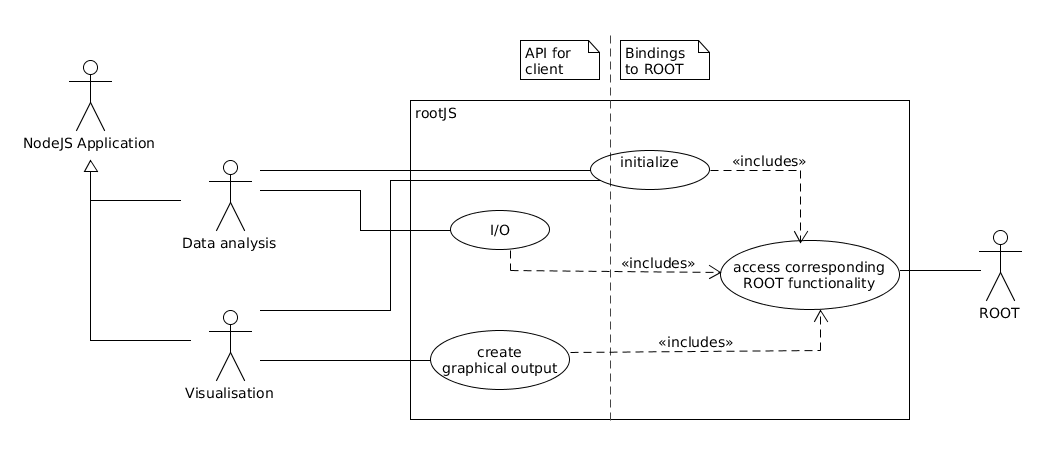
\includegraphics[width=18cm]{./latex/resources/usecaseOverview.png}
	\caption{use case overview}
\end{figure}

\pagebreak[4]

\section{Object Models}
Figure 6.2 illustrates what the rootJS architecture may look like.\\
\textit{ROOTPrototype::init} uses V8 to create an interface to the available variables, functions and classes of ROOT for a client Node.js application.
Functions provided through this interface internally call \textit{methodProxy} to determine the associated ROOT function through the given function name of the callee. This allows handling of supplied callback functions by passing them via the \textit{args} parameter.\\
Constructor functions provided by the interface internally use \textit{classProxy} instead of \textit{methodProxy} on calls to generate matching JavaScript object through the \textit{ProxyObjectFactory}.
Every \textit{ROOT:PrototypeObject} provides the \textit{globalGetter} and \textit{globalSetter} methods to interface with ROOT's global variables. Again the \textit{ProxyObjectFactory} will be used to generate needed JavaScript objects.
\\ \\
The \textit{ProxyObjectFactory} instantiates a class realizing the \textit{ProxyObject} interface. The actual class type will be decided by using the \textit{type} parameter.
If the \textit{ProxyObject} contains a scalar type (like int, long, string, etc.) the \textit{getV8Handle} method will simply return the corresponding \textit{v8::handle} with the value at a defined address.
If the \textit{ProxyObject} contains an object, \textit{getV8Handle} will recursively call the \textit{ProxyObjectFactory} for every element it contains to finally build the encapsulating JavaScript object.
To handle cyclic references a caching mechanism that stores already created \textit{v8::handle}s is used.

\begin{figure}[htb]
	\centering
	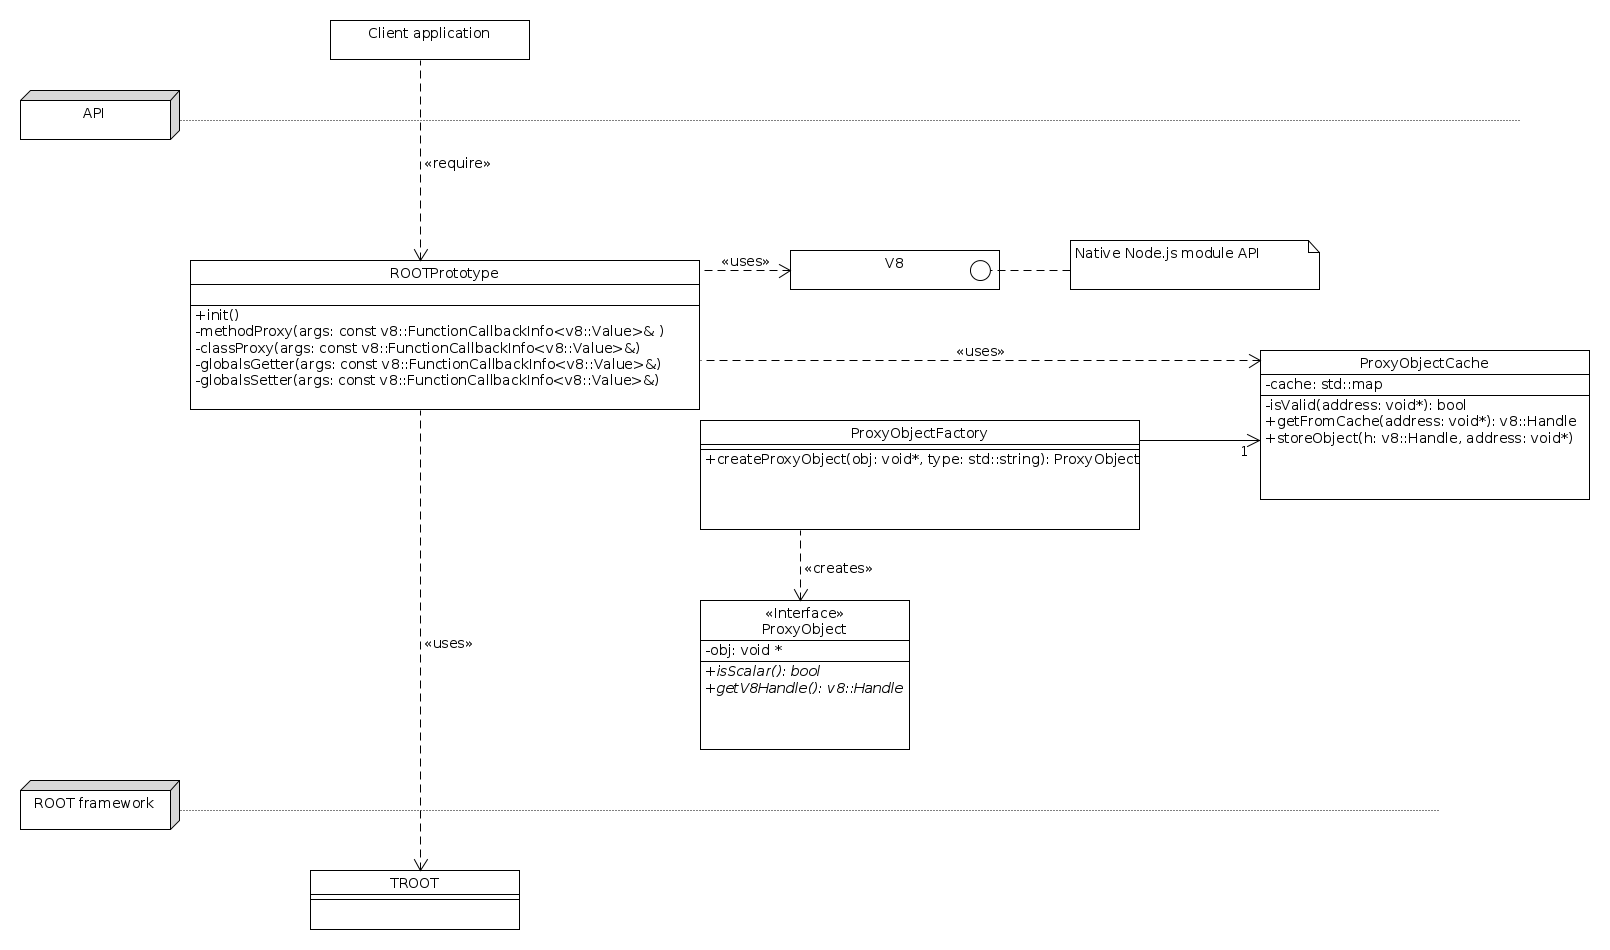
\includegraphics[width=18cm]{./latex/resources/architecture.png}
	\caption{basic architecture draft}
\end{figure}

\pagebreak[4]

\section{Dynamic Models}
The following figure shows how rootJS initializes upon being called the first time by a client application. As bindings do not add any functionality of their own, the client application is not further specified. After the bindings are initialized the client application may use any ROOT functionality through the roootJS API.
\begin{figure}[htb]
	\centering
	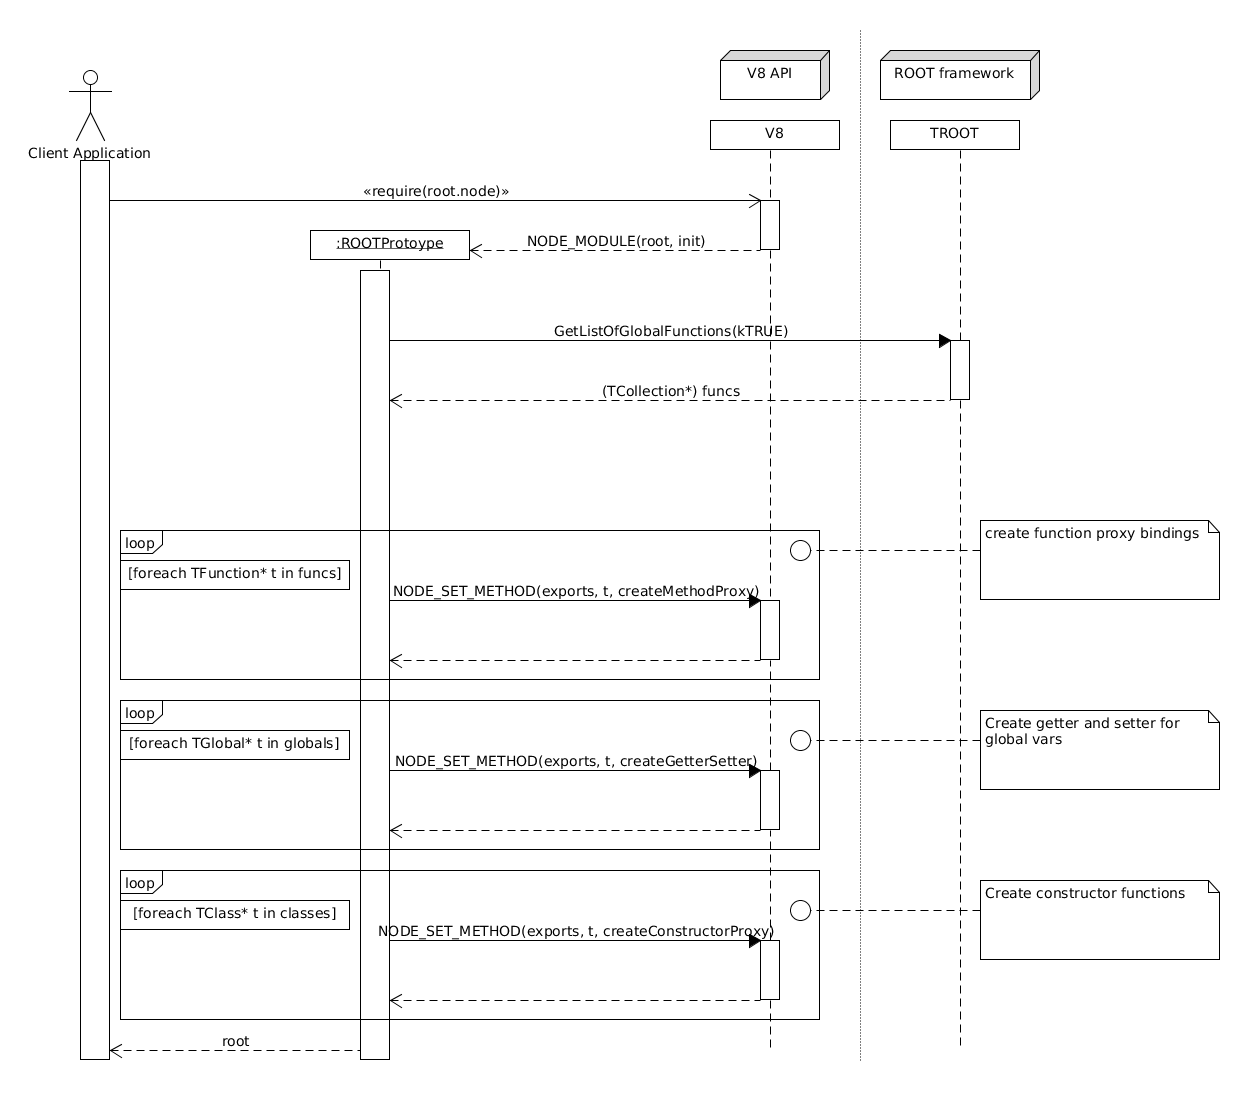
\includegraphics[width=18cm]{./latex/resources/startupSequence.png}
	\caption{basic startup sequence}
\end{figure}
